\documentclass[11pt]{article}
\usepackage{amssymb, amsmath, subcaption, cite,url,bm}
\usepackage{graphicx}
\usepackage{mathtools}
\usepackage[a4paper, total={6.7in, 8in}]{geometry}
\setlength{\textheight}{8.5in} \setlength{\topmargin}{-.2in}
\setlength{\headheight}{.2in} \setlength{\headsep}{0in}
\setlength{\parskip}{0.12in}
\setlength\parindent{0pt}
\title{{\bf Fundamentals of Geometry Project 2}\\Coloring Gaussian Curvature on Quartic Triangular B\'ezier Patches\\ From Smooth Approximations of Irregular Closed Blender Meshes\vspace{-0.25in}}
\author{Brandon Drumheller, Adam Freeman}
\date{\vspace{-0.25in}May 19, 2016}


\DeclarePairedDelimiter\abs{\lvert}{\rvert}%
\DeclarePairedDelimiter\norm{\lVert}{\rVert}%

% Swap the definition of \abs* and \norm*, so that \abs
% and \norm resizes the size of the brackets, and the 
% starred version does not.
\makeatletter
\let\oldabs\abs
\def\abs{\@ifstar{\oldabs}{\oldabs*}}
%
\let\oldnorm\norm
\def\norm{\@ifstar{\oldnorm}{\oldnorm*}}
\makeatother

\newcommand*{\Value}{\frac{1}{2}x^2}%

\begin{document}
	\maketitle
	%Title of the project%
	\section*{Project Description:}
	\vspace{-0.2in} 
	The goal of this project was to color Gaussian curvature on quartic B\'ezier Patches. These patches were generated from smooth approximations of arbitrary closed meshes, created in the open source modeling program Blender. The refinement process follows the algorithm detailed by Loop \cite{loop1994smooth}. 
	
	\subsection*{Spline Construction:}
	The spline construction is split into three stages, each of  which is briefly detailed and illustrated:
	\vspace{-0.1in}
	\begin{enumerate}
		\item Mesh Refinement
		\item Quad-Net Construction
		\item Quartic Triangular B\`ezier Patch Construction
	\end{enumerate}
	This output of this algorithm is a collection of quartic triangular B\`ezier patches.
	
	\subsubsection*{Mesh Refinement}
	The refined meshes are a ``smoothing" of the the inputted closed meshes. The meshes resulting from this step have the property that each vertex in the mesh has exactly 4 edges incident on it. As the process is computationally expensive for complex meshes (as with $e$ edges and $v$ vertices  $\mathcal{O}(e\cdot v)$), simpler meshes are included for illustration.	
	\begin{figure}
			\centering
			\captionsetup{justification=centering}
			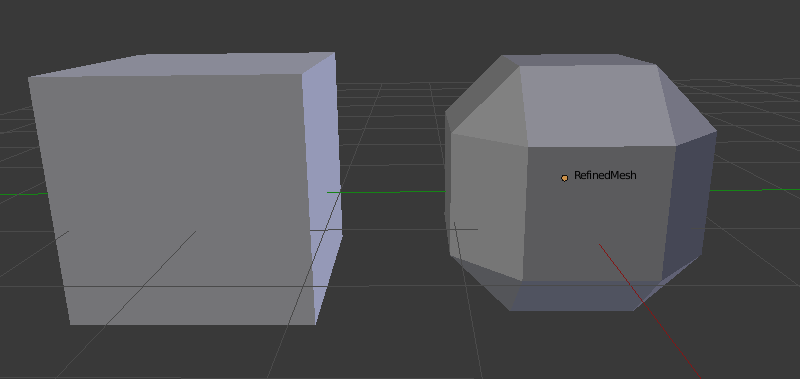
\includegraphics[width=.7\linewidth]{img/refine_cube}
			\caption{A cube (left) and the resulting refined mesh $\mathcal{M}^1$ (right).}
	\end{figure}	
	\begin{figure}
		\centering
		\captionsetup{justification=centering}
		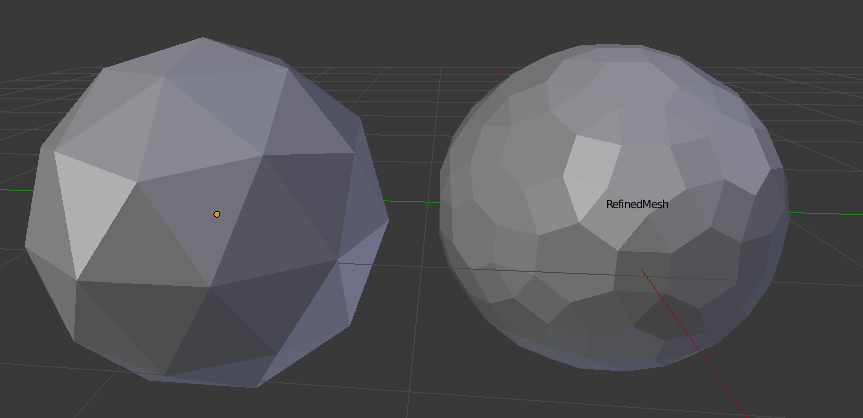
\includegraphics[width=.7\linewidth]{img/refine_icosphere}
		\caption{An icosphere (left) and the resulting refined mesh $\mathcal{M}^1$ (right).}		
	\end{figure}
	\begin{figure}
		\centering
		\captionsetup{justification=centering}
		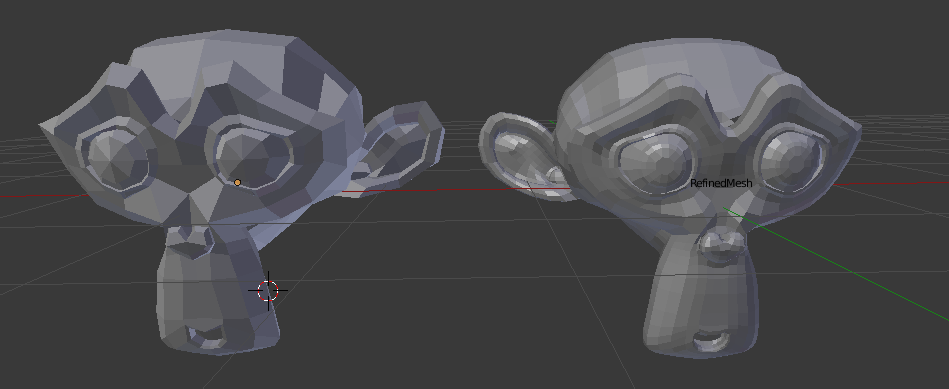
\includegraphics[width=.7\linewidth]{img/refine_monkey}
		\caption{A monkey head (nicknamed `Suzanne' left) and the resulting refined mesh $\mathcal{M}^1$ (right).}			
	\end{figure}

	\pagebreak
	
	\subsubsection*{Quad-Net Construction}
	Quad-nets are a set of 16 points that surround each vertex. These points form nets that when ``stitched" together cover the entire refined mesh $\mathcal{M}^1$. Ultimately, the quad-nets serve as a intermediary phase between the mesh refinement and the generation of quartic triangular B\`ezier surface patches. 
	\begin{figure}[bp!]
		\centering
		\captionsetup{justification=centering}
		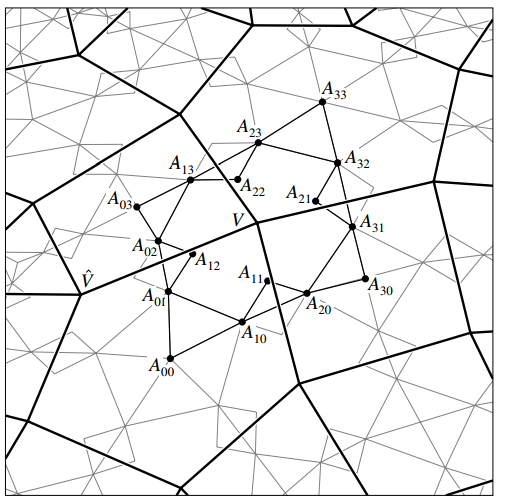
\includegraphics[width=.5\linewidth]{img/loop_quad_net}
		\caption{The quadnet corresponding to vertex $V$ on the refined mesh $\mathcal{M}^1$ \cite{loop1994smooth}.}			
	\end{figure} 	
	\begin{figure}[bp!]
		\vspace{0.35in}
		\centering
		\captionsetup{justification=centering}
		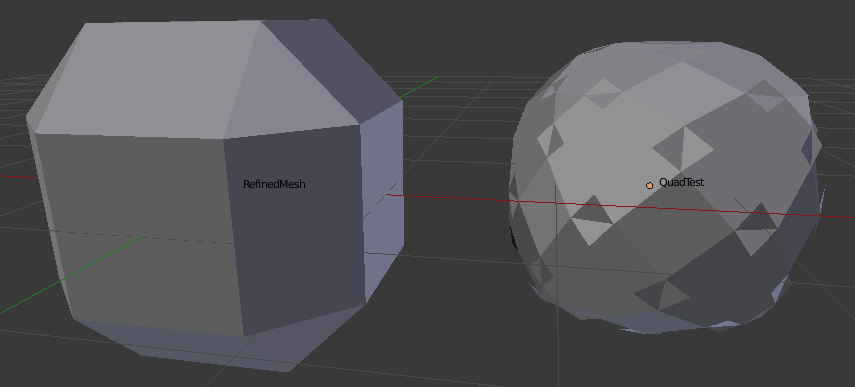
\includegraphics[width=.7\linewidth]{img/quad_cube}
		\caption{Quad-nets (right) corresponding to the cube's $\mathcal{M}^1$ (left)}	
	\end{figure}
	
	\pagebreak

	\begin{figure}[h]
		\centering
		\captionsetup{justification=centering}
		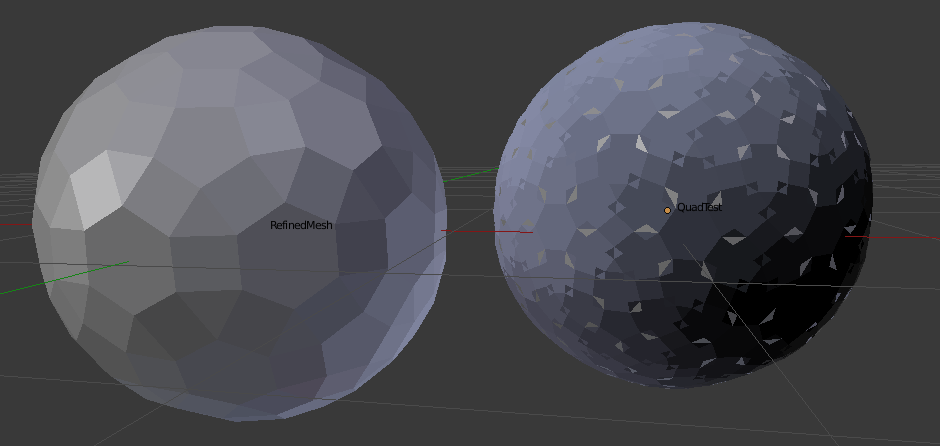
\includegraphics[width=.7\linewidth]{img/quad_icosphere}
		\caption{Quad-nets (right) corresponding to the icosphere's $\mathcal{M}^1$ (left)}	
	\end{figure}
	
	\vspace{0.25in}
	As previously stated, the implementation is contingent on the fact that the $\mathcal{M}^0$ is a closed mesh. Upon closer examination one finds that the monkey head `Suzanne' is an open mesh. Although the smoothing process succeeds, quad-net resolution fails for this open surface. \\

	\begin{figure}[h]
		\centering
		\captionsetup{justification=centering}
		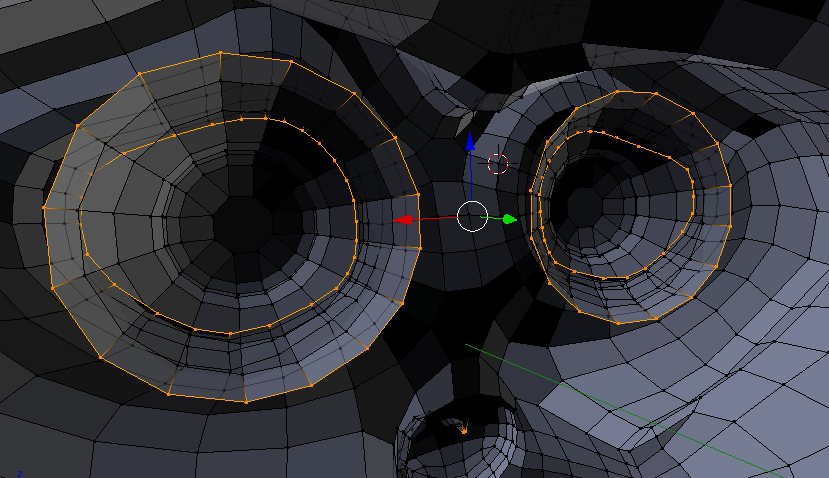
\includegraphics[width=.5\linewidth]{img/quad_monkey}
		\caption{Inside of `Suzanne'. Upon close examination one recognizes the mesh is open.}	
	\end{figure}
	
	\subsubsection*{Quartic Triangular B\`ezier Patch Construction}
	The final step of the construction creates a collection of triangular patch control points, from which unique equations for quartic triangular B\`ezier patches are calculated. From these patches the Gaussian curvature is calculated and colored.   
	
	Quartic triangular B\`ezier patches are calculated using the equation ($n=4$): 
	$$\bm{\sigma}(s,t,u) = \displaystyle \sum_{\begin{smallmatrix} i+j+k=n \\ i,j,k \ge 0\end{smallmatrix}} \frac{n!}{i!j!k!} s^i t^j u^k \alpha^i \beta^j \gamma^k \quad s + t + u = 1$$ 
	
	\pagebreak
	\begin{figure}[h]
		\centering
		\captionsetup{justification=centering}
		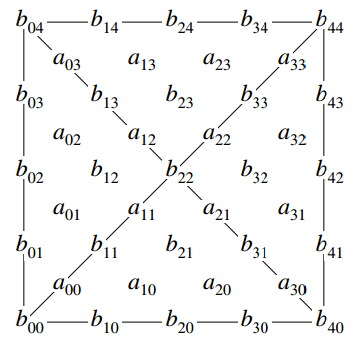
\includegraphics[width=.4\linewidth]{img/bezier_loop}
		\caption{The 4 triangular B\`ezier patches on a quad-net. \cite{loop1994smooth}}	
	\end{figure}
	
	\begin{figure}[h]
		\centering
		\captionsetup{justification=centering}
		\includegraphics[width=.45\linewidth]{img/quartic}
		\caption{Application of the above formula to the left triangular B\`ezier patch in Figure 8}
	\end{figure}
	
	\pagebreak
	
	\subsection*{Coloring Quartic B\`ezier Patches:}
	$\langle$add explanation of coloring process here$\rangle$
	
	\section*{Software:}
	\vspace{-0.20in}
	Blender, Python 3.5.1
	
	
	\section*{Images/animations produced:}
	$\langle$Add images and animations along with explanations here.$\rangle$
	
	\section*{Relevant concepts/equations/formulas covered in class:}
	\begin{enumerate}
		\item 	The unit normal to a surface patch $\bm{\sigma}$ used to calculate the Gaussian curvature. $$\vec{n} = \dfrac{\bm{\sigma}_u \times \bm{\sigma}_v}{\norm{\bm{\sigma}_u \times \bm{\sigma}_v}}$$ 
		\item The first fundamental form coefficient used to calculate the Gaussian curvature. 
		$$E = \bm{\sigma}_u \cdot \bm{\sigma}_u$$
		\item The first fundamental form coefficient used to calculate the Gaussian curvature. 
		$$F = \bm{\sigma}_u \cdot \bm{\sigma}_v$$
		\item The first fundamental form coefficient used to calculate the Gaussian curvature. $$G = \bm{\sigma}_v \cdot \bm{\sigma}_v$$
		\item The second fundamental form coefficient used to calculate the Gaussian curvature. $$L = \bm{\sigma}_{uu} \cdot \vec{n}$$
		\item The second fundamental form coefficient used to calculate the Gaussian curvature. $$M = \bm{\sigma}_{uv} \cdot \vec{n}$$
		\item The second fundamental form coefficient used to calculate the Gaussian curvature.$$N = \bm{\sigma}_{vv} \cdot \vec{n}$$		
		\item The Gaussian curvature. $$K = \dfrac{LN-M^2}{EG-F^2}$$
		\item The formulation of quartic B\`ezier patches for control pts $\alpha^i, \beta^j, \gamma^k $ $$\displaystyle \bm{\sigma}(s,t,u) = \sum_{\begin{smallmatrix} i+j+k=n \\ i,j,k \ge 0\end{smallmatrix}} \frac{n!}{i!j!k!} s^i t^j u^k \alpha^i \beta^j \gamma^k \quad s + t + u = 1$$
	\end{enumerate}
		
	\bibliography{proj2}
	
	\bibliographystyle{plain}
	
	\nocite{blender}
	\nocite{python}
	\nocite{drawio}
	
\end{document}